\chapter{Aspects énergétiques et corrélation}
	
	Jusqu'ici, nous avons négligé les notions de puissance et l'énergie, qui sont des caractéristiques essentielles dans l'analyse des signaux. Elles ont un intérêt pratique dans de nombreux domaines d'ingénierie car elles quantifient le travail effectué par un système physique (que ce soit dans les systèmes électriques, mécaniques, de télécommunications ...).	  
	En traitement du signal, elles ont un intérêt supplémentaire. Dans de nombreux cas pratiques, on ne dispose pas de l'expression exacte de la transformée de Fourier d'un signal. Par contre on connait la répartition de l'énergie ou de la puissance en fonction de la fréquence. Ces termes sont appelés densité spectrale en puissance ou en énergie.
	Dans ce chapitre, nous allons voir qu'à partir de l'expression temporelle du signal, on peut toujours remonter à ces densités. Pour cela, nous allons introduire une nouvelle notion : la corrélation. Elle présente un autre intérêt pratique : la mesure du degré de ressemblance entre deux signaux. 
	
	Dans certains cas, que vous rencontrerez dans les cours de signaux aléatoires, les expressions exactes des signaux ne sont pas disponibles. Nous allons voir dans ce chapitre que la corrélation va nous permettre de déterminer la manière dont la puissance ou l'énergie est répartie dans le domaine fréquentiel. Ces notions nous permettront aussi de déterminer l'impact du système sur le transfert d'énergie ou de puissance. 
	
	\section{Définitions de la puissance et de l'énergie d'un signal}
	Selon leur nature, les signaux transportent une énergie, que l'on peut quantifier soit sous la forme de puissance, soit sous la forme d'énergie. Nous allons préciser ici les définitions de ces grandeurs.
	
	\subsection{Puissance}
	La puissance correspond à la quantité d'énergie transportée par un signal pendant une unité de temps donnée. Celle-ci peut varier au cours du temps. On parle alors de puissance instantanée. Avant de préciser sa définition, considérons l'exemple d'un signal électrique, caractérisé par un courant ou par une tension. Soit une résistance R traversée par un courant i(t), avec une tension u(t) à ses bornes. La puissance instantanée p(t) du signal, et fournie à la résistance, est donnée par \ref{puissance_elec_resistance}.
	\begin{equation}\label{puissance_elec_resistance}
	p(t)=\frac{u(t)^{2}}{R}=Ri(t)^{2}
	\end{equation}
	
	On remarque que la puissance est obtenue en élevant au carré la grandeur physique formant le signal (ici, la tension ou le courant). La puissance est donc une grandeur quadratique. Dans le cas précédent, la puissance électrique dépend de la résistance électrique R. On pourrait s'affranchir de cette dernière en considérant une résistance unitaire, normalisant ainsi la puissance.
	
	De manière générale, la puissance instantanée p(t) d'un signal temporel quelconque défini par une fonction f(t) est le carré de cette fonction (\ref{Def_puissance_instantanée}). La puissance est définie en Joules/s ou, de manière plus courante, en Watts (W). Dans le cas d'un signal complexe, on doit considérer le module.
	\begin{equation}\label{Def_puissance_instantanée}
	p(t)=f(t)^{2}
	\end{equation}
	\begin{equation}\label{Def_puissance_instantanée_complexe}
	p(t)=|f(t)|^{2}
	\end{equation}
	
	La puissance instantanée étant fluctuante dans le temps, d'autres manières de mesurer cette puissance sont souvent requises en pratique. On peut par exemple définir la puissance moyenne d'un signal $\overline{P}$ à l'aide de \ref{Def_puissance_moy}. Ce n'est rien d'autre que la moyenne temporelle de la puissance instantanée.
	\begin{equation}\label{Def_puissance_moy}
	\overline{P}=\lim_{T \to +\infty}\frac{1}{2T}\int_{-T}^{+T}|f(t)|^{2}dt
	\end{equation}
	

	\subsection{Energie}
	D'après la définition de la puissance, l'énergie transportée par un signal est liée à la puissance instantanée. L'énergie E transportée par un signal pendant une période délimitée par $t_{1}$ et $t_{2}$ est donnée par \ref{Def_energie}. Son unité est le Joule (J).
	\begin{equation}\label{Def_energie}
	E=\int_{t_{1}}^{t_{2}}p(t)dt=\int_{t_{1}}^{t_{2}}|f(t)|^{2}dt
	\end{equation} 
	
	L'énergie totale du signal se calcule donc à l'aide de la relation \ref{Def_energie}, en l'intégrant sur tout le domaine de définition du signal.
	\begin{equation}\label{Def_energie_tot}
	E_{tot}=\int_{-\infty}^{+\infty}p(t)dt=\int_{-\infty}^{+\infty}|f(t)|^{2}dt
	\end{equation}
	
	On peut aussi relier l'énergie totale à la puissance moyenne à l'aide de la relation suivante.
	\begin{equation}\label{key}
	E_{tot}= \lim_{T \to +\infty}\overline{P} \cdot 2T=\lim_{T \to +\infty}\int_{-T}^{+T}|f(t)|^{2}dt
	\end{equation}
	
	
	\subsection{Signaux à énergie/puissance finie}
	Les signaux peuvent être classés en deux catégories en prenant comme critère leur énergie. Si l'équation \ref{Def_energie_tot} donnant l'énergie totale du signal converge, alors le signal est dit à énergie finie. C'est notamment le cas des signaux apériodiques et à supports temporels bornés. Ces signaux ont cependant une puissance moyenne qui tend vers zéro. Ils ne peuvent donc pas être caractérisés par leur puissance moyenne.
	
	Si l'équation \ref{Def_energie_tot} ne converge pas, on ne peut pas caractériser le signal par son énergie totale. On utilise alors la puissance moyenne, qui sera toujours finie. On parle alors de signaux à puissance finie. C'est notamment le cas des signaux périodiques ou de signaux apériodiques à support temporel non borné (signaux aléatoires). Comme ils sont à support infini, leur énergie l'est aussi. Par contre, on retrouve la puissance moyenne sur une période T du signal, donnée par \ref{Pmoy_signal_periodique}. 
	\begin{equation}\label{Pmoy_signal_periodique}
	\overline{P}=\frac{1}{T}\int_{-\frac{T}{2}}^{+\frac{T}{2}}f(t)^{2}dt
	\end{equation}
	
	

	
	\section{Calcul de la puissance dans le domaine fréquentiel}
	
	Dans la partie précédente, nous avons défini la puissance d'un signal directement à partir de son expression dans le domaine temporel. Dans cette partie, nous allons voir comment les calculer à partir de l'expression du signal dans le domaine fréquentiel. 
	
	\subsection{Densité spectrale d'amplitude}
	
	Revenons sur l'unité de l'amplitude de l'amplitude ou module de la transformée de Fourier (ou spectre) d'un signal non périodique. S'il est périodique, le résultats de la transformée de Fourier est un spectre de raies; l'unité de l'amplitude du spectre est la même que le signal. Le spectre indique alors directement la distribution de l'amplitude dans le domaine fréquentiel.
	
	Ce n'est pas le cas pour un signal non périodique. Pour un signal f(t), sa transformée de Fourier F(f) lui est reliée par la transformée de Fourier inverse :
	
	\begin{equation}\label{key}
	f(t)=\int_{-\infty}^{+\infty}F(f)e^{j2\pi ft}df
	\end{equation}
	
	Pour assurer l'homogénéité des unités, F(f) ne peut pas avoir la même unité que f(t), puisque f(t) est le résultat de l'intégration du spectre sur un intervalle de fréquence. Le le module de F(f) est une densité spectrale en amplitude. Par exemple, si le signal f(t) est une tension exprimée en V, le module de sa transformée de Fourier |F(f)| représente une densité spectrale de tension exprimée en V/Hz (ou $V/rad.s^{-1}$ si on considère une pulsation au lieu d'une fréquence). Cette notion de densité spectrale d'amplitude se comprend : le spectre permet d'analyser la répartition de l'amplitude du signal dans le domaine fréquentiel. Déterminer l'amplitude du signal sur une plage de fréquence donnée revient à intégrer la transformée de Fourier du signal sur cet intervalle de fréquence. C'est ce qu'illustre la figure \ref{Fig:Densite_spectrale_amplitude}.
	
	\begin{figure}[h!]
		\centering
		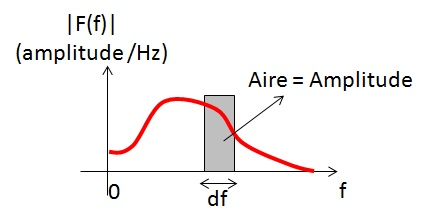
\includegraphics[scale=0.6]{images/Densite_spectrale_amplitude.jpg}
		\caption{Densité spectrale d'amplitude}	
		\label{Fig:Densite_spectrale_amplitude} 
	\end{figure}
	 
	
	
	\subsection{Cas des signaux périodiques - Egalité de Parseval}
	On considère un signal périodique f(t) de période $T_{0}$ avec $f_{0}=\frac{1}{T_{0}}$. Ce signal peut être décomposé en une série de Fourier, selon \ref{decompo_serie_Fourier}. L'ensemble des coefficients de Fourier F(n) peuvent être représentés sous la forme d'un spectre de raies d'amplitude, comme le montre la figure \ref{Fig:spectre_raies_ampl_puissance}.
	\begin{equation}\label{decompo_serie_Fourier}
	f(t)=\sum_{n=-\infty}^{+\infty}f_{n}(t)=\sum_{n=-\infty}^{+\infty}F(n)e^{jn2\pi f_{0}t}
	\end{equation}
	Chaque membre $f_{n}(t)$ de la série de Fourier transporte une partie de la puissance du signal. La puissance moyenne $P_{n}$ de chacun de ces membres peut être reliée au coefficient de Fourier selon \ref{Pmoy_term_fourier}.
	\begin{equation}\label{Pmoy_term_fourier}
	P_{n}=\frac{1}{T_{0}}\int_{T_{0}}|f_{n}(t)|^{2}dt=\frac{1}{T_{0}}\int_{T_{0}}|F(n)|^{2}dt
	\end{equation}
	
	A partir de cette définition, une nouvelle représentation du spectre est possible : un spectre de puissance où chaque raie porte une puissance $P_{n}$. Celui-ci permet d'indiquer la répartition de la puissance dans le domaine spectral (figure \ref{Fig:spectre_raies_ampl_puissance}).
	
	\begin{figure}[h!]
		\centering
		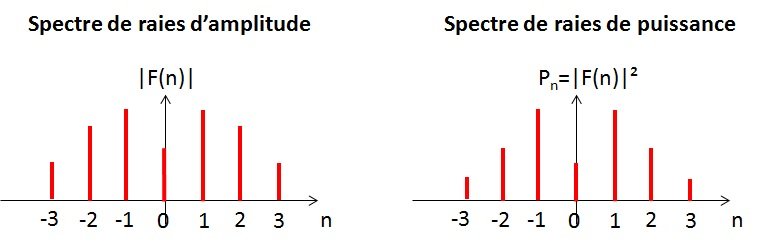
\includegraphics[scale=0.6]{images/spectre_raies_ampl_puissance.jpg}
		\caption{Spectre de raies d'amplitude et de puissance pour un signal périodique}	
		\label{Fig:spectre_raies_ampl_puissance} 
	\end{figure}

	La puissance moyenne du signal peut aussi être exprimée en fonction des coefficients de Fourier : il s'agit de l'égalité de Parseval (pour un signal périodique), donnée par \ref{Parseval_periodique}. La puissance moyenne est donc égale à la somme du module au carré de chaque coefficient du spectre. En d'autres termes, la puissance moyenne est la somme des différentes raies de puissance.
	\begin{equation*}
	\overline{P}=\frac{1}{T}\int_{T_{0}}|f(t)|^{2}dt=\frac{1}{T}\int_{T_{0}}|\sum_{n=-\infty}^{+\infty}f_{n}(t)|^{2}dt=\frac{1}{T}\int_{T_{0}}\sum_{n=-\infty}^{+\infty}|F(n)|^{2}dt
	\end{equation*}
	\begin{equation}\label{Parseval_periodique}
	\overline{P}=\sum_{n=-\infty}^{+\infty}|F(n)|^{2}
	\end{equation}
	
 	
	\subsection{Cas des signaux non périodiques - Densité spectrale de puissance}
	
	Considérons un signal f(t) quelconque. Le module de sa transformée de Fourier |F(f)| représente une densité spectrale d'amplitude. Chaque portion du spectre transporte une partie de la puissance du signal. Pour caractériser la répartition de la puissance du signal dans le domaine fréquentiel, on introduit la notion de densité spectrale de puissance du signal, notée $S_{F}(f)$, qui est le carré du module de la transformée de Fourier du signal (\ref{dsp}). La densité spectrale de puissance est exprimée en W/Hz (ou en $W/rad.s^{-1}$).
	\begin{equation}\label{dsp}
	S_{F}(f)=|F(f)|^{2}=F(f)\cdot F(f)^{*}
	\end{equation}
	
	A partir de cette définition, on remarque qu'intégrer la densité spectrale de puissance sur un intervalle de fréquence revient à calculer une puissance.
	Cependant, la notion de densité spectrale de puissance n'a de sens que pour les signaux à puissance finie, comme les fonctions périodiques ou à support temporel non borné. Pour les signaux à énergie finie, il est préférable d'utiliser une répartition fréquentielle donnée en densité spectrale d'énergie.
	
	\vspace{0.5\baselineskip}
	
	Le théorème de Parseval peut être étendu au cas des signaux non périodiques. Dans le cas où le signal est à énergie finie, il permet de calculer l'énergie totale du signal à partir de sa densité spectrale d'énergie (\ref{Parseval_non_periodique_Efinie}). En l'intégrant sur tout l'espace des fréquences, on détermine l'énergie totale du signal. Si le signal est à puissance finie, la puissance moyenne peut être calculée à partir de sa densité spectrale de puissance (\ref{Parseval_non_periodique_Pfinie}).
	
	\begin{equation}\label{Parseval_non_periodique_Efinie}
	E_{tot}= \lim_{T \to +\infty}\int_{-T}^{+T}|f(t)|^{2}dt=\int_{-\infty}^{+\infty}|F(f)|^{2}df
	\end{equation}
	
	\begin{equation}\label{Parseval_non_periodique_Pfinie}
	\overline{P}= \lim_{T \to +\infty}\frac{1}{2T}\int_{-T}^{+T}|f(t)|^{2}dt=\int_{-\infty}^{+\infty}|F(f)|^{2}df
	\end{equation}

	
	
	\section{Corrélation}

	
	\subsection{Définition}
	Comment comparer deux signaux ? Comment mesurer leur ressemblance ?  
	
	Une première tentative de définition d'une telle grandeur consiste à utiliser les outils dont nous disposons, par exemple le produit scalaire. Dans un premier temps, nous considérons des signaux bornés dans le temps sur un intervalle $[t_{1};t_{2}]$. Ce produit correspond à la moyenne temporelle de la multiplication des deux signaux à comparer $s_{1}$ et $s_{2}$, définie par la relation ci-dessous.
	
	\begin{equation*}
	\frac{1}{t_{2}-t_{1}}\int_{t_{1}}^{t_{2}}s_{1}(t)s_{2}(t)dt
	\end{equation*}
	
	La figure \ref{Fig:ressemblance_via_produit_scalaire} présente deux exemples permettant d'estimer l'intérêt de cette définition. A gauche, deux fonctions portes de même largeur apparaissent en même temps. La définition précédente renvoie une valeur maximale, indiquant une très grande ressemblance entre les deux signaux. A droite, on a décalé le signal $s_{2}$ par rapport $s_{1}$. Ils se ressemblent autant que dans le cas précédent, seul un délai a été ajouté entre eux. Pourtant, l'indicateur de ressemblance utilisé renvoie une valeur nulle que nous interprétons comme une faible corrélation.
	\begin{figure}[h!]
		\centering
		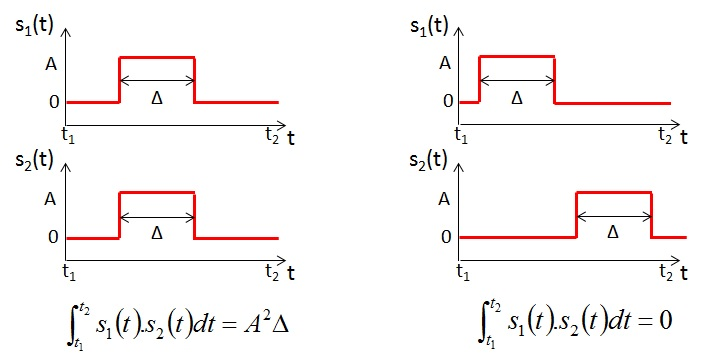
\includegraphics[scale=0.5]{images/ressemblance_via_produit_scalaire.jpg}
		\caption{Mesure du degré de "ressemblance" entre deux signaux par le produit scalaire}	
		\label{Fig:ressemblance_via_produit_scalaire} 
	\end{figure}
	
	La définition choisie n'est pas satisfaisante car elle prend en compte la position relative des deux signaux. Une astuce consiste à refaire le même calcul, mais pour différentes positions relatives entre les deux signaux, que nous noterons $\tau$. L'expression est donnée par \ref{Prod_conv_support_fini}. L'indicateur calculé correspond à la corrélation $R(\tau)$ entre ces deux signaux. Il n'est pas à valeur unique puisqu'il dépend de $\tau$. De manière générale, lorsqu'on travaille avec des signaux complexes, il est nécessaire de prendre le conjugué du signal $s_{2}$. Dans le cas où le signal est à support temporel infini (signal à puissance finie), la relation prend la forme \ref{Prod_conv_support_infini}.
	
	\begin{equation}\label{Prod_conv_support_fini}
	R(\tau)=\frac{1}{t_{2}-t_{1}}\int_{t_{1}}^{t_{2}}s_{1}(t)s^{*}_{2}(t-\tau)dt
	\end{equation}
	\begin{equation}\label{Prod_conv_support_infini}
	R(\tau)=\lim_{T \to \infty}\frac{1}{T}\int_{-\frac{T}{2}}^{+\frac{T}{2}}s_{1}(t)s^{*}_{2}(t-\tau)dt
	\end{equation}
	
	Dans le cas où les fonctions sont périodiques et de même période $T_{0}$, le calcul de la corrélation est donné par la relation ci-dessous.
	\begin{equation}\label{Prod_conv_periodique}
	R(\tau)=\frac{1}{T_{0}}\int_{t_{1}}^{t_{1}+T_{0}}s_{1}(t)s^{*}_{2}(t-\tau)dt
	\end{equation}
	
	Lorsque les signaux sont à énergie finie, la division par T n'est pas indispensable, sinon la corrélation risque de tendre vers 0. La définition (\ref{Correlation_E_fini}) est préférable.
	\begin{equation}\label{Correlation_E_fini}
	R(\tau)=\lim_{T \to \infty}\int_{-\frac{T}{2}}^{+\frac{T}{2}}s_{1}(t)s^{*}_{2}(t-\tau)dt
	\end{equation}
	 
	
	Reprenons l'exemple précédent et calculons la corrélation entre deux signaux pour vérifier la pertinence de cet indicateur. On décale la position respective du signal $s_{2}$ par rapport au signal $s_{1}$. Pour chaque position, on calcule la corrélation. Le résultat est présenté sur la figure \ref{Fig:ressemblance_via_convolution}. La corrélation est maximale lorsque $\tau = 0$, c'est-à-dire lorsque l'on superpose $s_{1}$ et $s_{2}$. Dès que l'on décale $s_{2}$ vers la droite ou vers la gauche, la corrélation décroit jusqu'à devenir minimale lorsque les deux signaux ne se recouvrent plus. L'indicateur définit fournit une meilleure mesure du degré de ressemblance entre deux signaux.  
	
	\begin{figure}[h!]
		\centering
		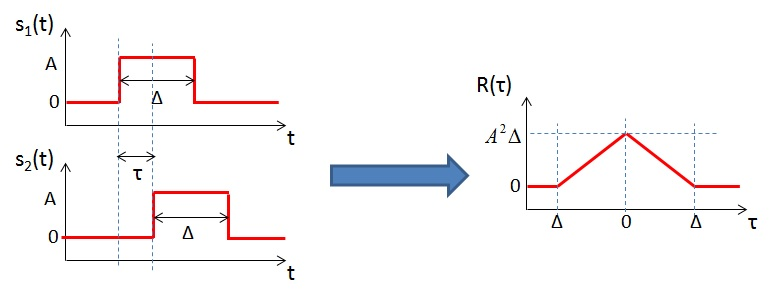
\includegraphics[scale=0.6]{images/ressemblance_via_convolution.jpg}
		\caption{Corrélation entre deux signaux}	
		\label{Fig:ressemblance_via_convolution} 
	\end{figure}

	On remarque que le calcul de la corrélation est assez proche de celui du produit de convolution. En effet, dans les deux cas, il s'agit d'un calcul d'une intégrale appliqué à un produit de deux signaux que l'on décale. La seule différence est qu'on ne "retourne" pas un des deux signaux, comme le montre le rappel des deux formules ci-dessous.
	\begin{figure}[h!]
		\centering
		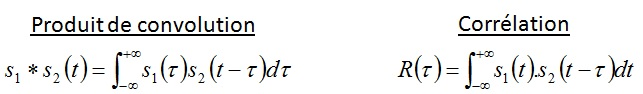
\includegraphics[scale=0.6]{images/convo_vs_correlation.jpg} 
	\end{figure}

	On peut exprimer le calcul de la corrélation sous la forme d'un produit de convolution, comme le montre \ref{equiv_conv_corr} :
	\begin{equation}\label{equiv_conv_corr}
	R(\tau)=\int_{-\infty}^{+\infty}s_{1}(t)s_{2}^{*}(t-\tau)dt=s_{1}*s_{2}(-\tau)
	\end{equation}

	
	Si on analyse ce que représente la corrélation, on remarque qu'elle est équivalente à une puissance. En effet, il s'agit d'une grandeur quadratique. Nous verrons plus loin qu'elle est intimement liée à la puissance des signaux.
	
	
	\subsection{Autocorrélation et intercorrélation}
	
	Selon les signaux considérés dans le calcul de corrélation, on distinguera deux cas :
	\begin{itemize}
		\item si le calcul s'effectue sur le même signal ($s_{1} = s_{2}$), on parlera d'autocorrélation que l'on notera $R_{11}(\tau)$
		\item si le calcul s'effectue sur deux signaux différents, on parlera d'intercorrélation que l'on notera $R_{12}(\tau)$.
	\end{itemize}

	L'autocorrélation permet de mesurer le degré de ressemblance d'un signal à une version décalée de lui-même. Comme nous allons le voir plus tard dans le cours, cela peut avoir de nombreuses applications comme la détection de composantes périodiques.
	
	L'intercorrélation permet de mesurer le degré de ressemblance entre deux signaux. Si deux signaux sont complètement décorrélés, alors leur intercorrélation restera minimale quelle que soit le décalage temporel que l'on applique entre ces deux signaux.
	
	
	\subsection{Propriétés de la corrélation}
	
	\subsubsection{Changement de variable}
	
	On démontre que :
	\begin{equation}\label{key}
	R_{11}(\tau)=\frac{1}{T}\int_{-\infty}^{+\infty}f(t)f^{*}(t-\tau)dt=\frac{1}{T}\int_{-\infty}^{+\infty}f(t+\tau)f^{*}(t)dt
	\end{equation}
	En effet, retarder la première fonction revient à avancer la seconde. Cette même propriété se retrouve pour la fonction d'intercorrélation.
	\begin{equation}\label{key}
	R_{12}(\tau)=\frac{1}{T}\int_{-\infty}^{+\infty}f_{1}(t)f^{*}_{2}(t-\tau)dt=\frac{1}{T}\int_{-\infty}^{+\infty}f_{1}(t+\tau)f^{*}_{2}(t)dt
	\end{equation}
	
	\subsubsection{Parité}
	La fonction d'autocorrélation est une fonction paire. En effet, on peut montrer que :
	\begin{equation}\label{key}
	R^{*}_{11}(-\tau)=\frac{1}{T}\int_{-\infty}^{+\infty}f^{*}(t)f(t+\tau)dt=\frac{1}{T}\int_{-\infty}^{+\infty}f^{*}(t-\tau)f(t)dt=\frac{1}{T}\int_{-\infty}^{+\infty}f(t)f^{*}(t-\tau)dt=R_{11}(\tau)
	\end{equation}
	
	Par contre, ce n'est pas nécessairement le cas pour la fonction d'intercorrélation.
	
	\subsubsection{Valeur à l'origine}
	Lorsqu'on analyse la formule de l'autocorrélation à l'origine ($\tau=0$), on retrouve la formule de la puissance moyenne pour les signaux à puissance finie(\ref{Def_puissance_moy}) ou celle de l'énergie totale pour les signaux à énergie finie (\ref{Def_energie_tot}). A partir du théorème de Parseval, on peut donner les valeurs à l'origine de la fonction d'autocorrélation :
	
	\begin{itemize}
		\item signal périodique : $R_{11}(0)=\overline{P}=\frac{1}{T}\int_{T}|f(t)|^{2}dt=\sum_{n=-\infty}^{+\infty}|F(n)|^{2}$
		\item  signal non périodique à puissance finie : $R_{11}(0)=\overline{P}=\lim_{T \to +\infty}\frac{1}{2T}\int_{-T}^{+T}|f(t)|^{2}dt=\int_{-\infty}^{+\infty}|F(f)|^{2}df$
		\item signal à énergie finie : $R_{11}(0)= E_{tot}=\lim_{T \to +\infty}\int_{-T}^{+T}|f(t)|^{2}dt=\int_{-\infty}^{+\infty}|F(f)|^{2}df$		
	\end{itemize}


	\subsubsection{Valeur(s) maximale(s)}
	
	L'autocorrélation présente toujours un maximum à l'origine, pour $\tau = 0$, égale soit à la puissance moyenne, soit à l'énergie totale du signal.  On en déduit donc la propriété suivante :
	\begin{equation}\label{key}
	R_{11}(0) \geq R_{11}(\tau)
	\end{equation}
	
	Ce n'est pas forcément le cas pour la fonction d'intercorrélation.
	 
	La fonction d'autocorrélation peut présenter des maxima en d'autres points d'abscisse, notamment lorsque le signal est périodique. Pour un signal de période $T_{0}$, alors la fonction d'autocorrélation présente des maxima pour toutes les valeurs d'abscisse $\tau = k\cdot T_{0}$ où k est un nombre entier. Cette propriété fournit un des intérêt pratique de la fonction d'autocorrélation et de son tracé : elle permet de repérer des composantes périodiques dans un signal complexe. 
	
	Cet outil d'analyse du signal est illustré dans les deux exemples ci-dessous.\\
	
	\underline{\textbf{Exemple 1 : bruit blanc}}
	
	Par définition, un bruit est un signal aléatoire. Sa valeur à tout instant reste imprédictible. Selon la loi statistique suivie par ses valeurs, il peut être qualifié différemment : par exemple, on parle de bruit blanc gaussien si ses valeurs suivent une loi normale. Le qualificatif blanc vient de la répartition spectrale du signal, qui est quasiment constante quelle que soit la fréquence. Nous le comprendrons à la partie IV.
	Considérons un bruit blanc gaussien centré, c'est-à-dire de moyenne nulle. L'écart-type des valeurs prises par le signal est noté $\sigma$. Ce signal constitue un excellent modèle du bruit d'origine thermique affectant les composants électroniques et les récepteurs radio.
	
	La figure ci-dessous présente un exemple de simulation d'un tel bruit, avec $\sigma=0.5$ : en haut, le relevé temporel; en bas la fonction d'autocorrélation calculée. On remarque que la fonction d'autocorrélation est minimale pour toutes les valeurs de $\tau$, sauf pour $\tau = 0$. L'amplitude de ce pic est égale à $\sigma^{2} = 0.25$. Comme le signal est totalement aléatoire, comparer ce signal à une version décalée de lui-même revient à comparer deux signaux décorrélés. L'autocorrélation d'un tel signal peut être modélisée par une impulsion de Dirac.
	
	\begin{figure}[h!]
		\centering
		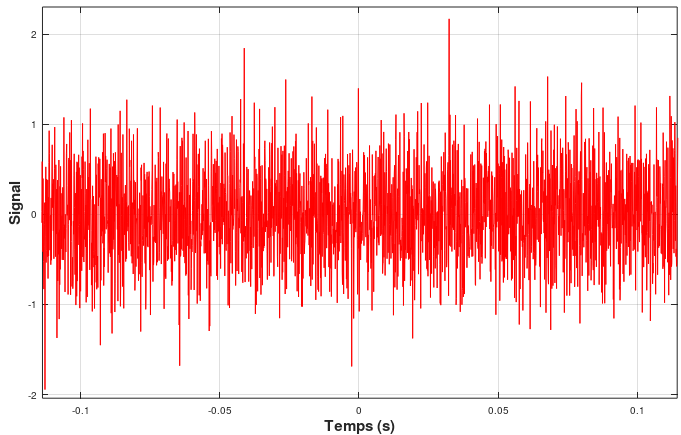
\includegraphics[scale=0.6]{images/Mesure_autocorr_bruit.png}
	\end{figure}
	
	\begin{figure}[h!]
		\centering
		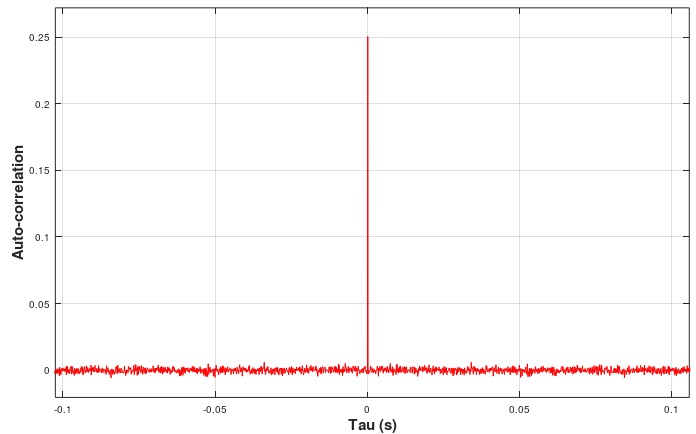
\includegraphics[scale=0.6]{images/Mesure_autocorr_bruit_2.png}
		\caption{Bruit blanc gaussien ($\sigma = 0.5$)(en haut) et sa fonction d'autocorrélation (en bas)}	
		\label{Fig:Mesure_autocorr_bruit} 
	\end{figure}
	
	
	

	
	
	
	
	\textbf{\underline{Exemple 2 : extraction d'une composante périodique dans un signal bruité}}
	
	 Dans ce deuxième exemple, on considère un signal fortement affecté par un bruit blanc gaussien. Un relevé temporel de ce signal est présenté à la figure \ref{Fig:Mesure_autocorr_1}. Ce signal aléatoire semble contenir une composante périodique, de période proche de 20 ms. Sa présence est clairement révélée par le tracé de la fonction d'autocorrélation du signal. On retrouve un fort pic à l'origine, lié à la présence du bruit blanc gaussien. Mais on ne retrouve pas une fonction d'autocorrélation minimale pour $|\tau| > 0$. On observe des maxima locaux se répétant périodiquement, tous les $\tau=k \cdot 0.02$ avec $k \in \mathbb{Z}$. Ce résultat confirme la présence d'une composante périodique de 20 ms cachée dans le signal.
	
	\begin{figure}[h!]
		\centering
		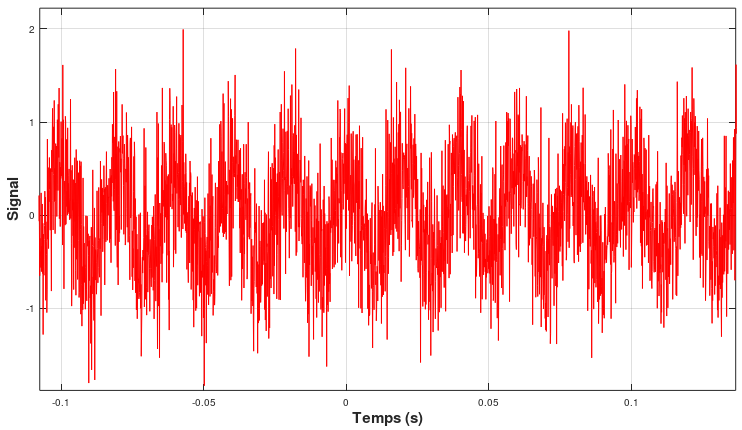
\includegraphics[scale=0.6]{images/Mesure_autocorr_1.png}
	\end{figure}

	\begin{figure}[h!]
		\centering
		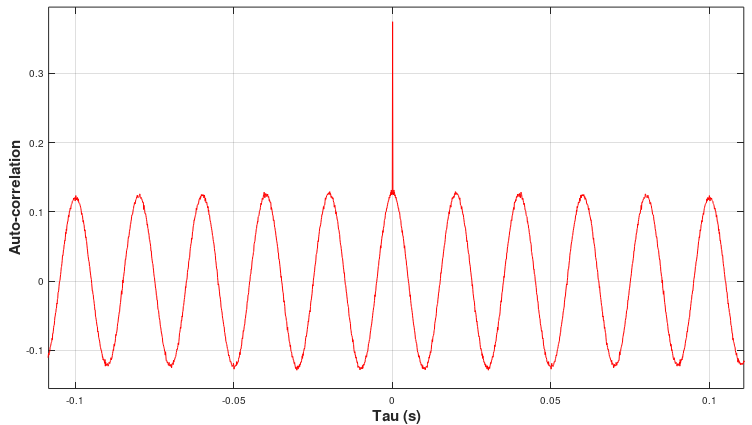
\includegraphics[scale=0.6]{images/Mesure_autocorr_2.png}
		\caption{Signal bruité (en haut) et analyse par son autocorrélation (en bas)}	
		\label{Fig:Mesure_autocorr_1} 
	\end{figure}
	
	\subsubsection{Valeur minimale}
	Puisqu'on aborde la question de la valeur maximale, on pourrait s'interroger sur la valeur minimale prise par la fonction de corrélation. On atteint un minimum lorsque les deux fonctions à comparer ne présentent aucune corrélation. On serait tenté de penser que la valeur prise par la corrélation est nulle, mais ce n'est pas le cas. La fonction de corrélation dépend aussi des amplitudes et des valeurs moyennes prises par les signaux. Comparer les valeurs minimales et maximales de deux fonctions de corrélation, calculées sur des signaux différents, avec des amplitudes et moyennes différentes, n'a pas de sens. Cela n'indiquera pas qu'il y a plus de corrélation dans un cas que dans un autre.
	
	
	\subsection{Exemples}
	
	\subsubsection{Exemple 1 : autocorrélation d'une fonction cosinusoïdale}
	
	On considère le signal périodique $s(t)=Acos(2\pi f_{0}t+\theta_{0})$, où $f_{0}$ est la fréquence du signal et $\theta_{0}$ sa phase initiale. Déterminez la fonction d'autocorrélation de ce signal et tracez son allure.
	
	La fonction d'autocorrélation est obtenue en calculant l'intégrale \ref{Prod_conv_periodique}. Celle-ci peut être résolue en utilisant la relation trigonométrique suivante : $cos(a)cos(b)=\frac{1}{2}[cos(a-b)+cos(a+b)]$.
	\begin{equation*}
	R_{11}(\tau)=\frac{1}{T_{0}}\int_{0}^{T_{0}}A^{2}cos(2\pi f_{0}t+\theta_{0})cos(2\pi f_{0}(t-\tau)+\theta_{0})dt~,~avec~T_{0}=\frac{1}{f_{0}}
	\end{equation*}
	\begin{equation*}
	R_{11}(\tau)=\frac{A^{2}}{2T_{0}}[\int_{0}^{T_{0}}cos(2\pi f_{0}\tau)dt+\int_{0}^{T_{0}}cos(2\pi f_{0}(2t-\tau)+2\theta_{0})dt]
	\end{equation*}
	Le second terme de l'équation étant une fonction périodique de t, son intégration sur une période renvoie une valeur nulle. La relation précédente se simplifie :
	\begin{equation*}
	R_{11}(\tau)=\frac{A^{2}}{2T_{0}}cos(2\pi f_{0}\tau)\int_{0}^{T_{0}}dt=\frac{A^{2}}{2}cos(2\pi f_{0}\tau)
	\end{equation*}
	
	L'allure de la fonction d'autocorrélation est présentée ci-dessous. La fonction est paire et présente plusieurs maxima : un pour $\tau=0$, mais aussi pour tous les multiples de la période $T_{0}$ du signal. Cela se comprend intuitivement : si on créé une réplique du signal que l'on décale d'un multiple de la période, lorsqu'on superpose le signal original et sa réplique, ceux-ci sont confondus. 
	\begin{figure}[h!]
		\centering
		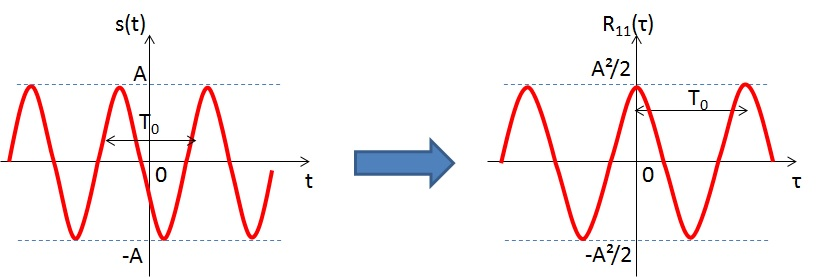
\includegraphics[scale=0.6]{images/autocorr_cosinus.jpg}
	\end{figure}
	
	La puissance moyenne du signal est donnée par : $\overline{P}=\frac{1}{T_{0}}\int_{0}^{T_{0}}A^{2}cos^{2}(2\pi f_{0}t+\theta_{0})dt=\frac{A^{2}}{2T_{0}}\int_{0}^{T_{0}}(1+cos(4\pi f_{0}t+\theta_{0}))dt=\frac{A^{2}}{2}$. On vérifie ainsi que la valeur maximale prise par la fonction d'autocorrélation à l'origine est égale à la puissance moyenne du signal.

	On peut aussi remarquer que l'effet de la phase du signal $\theta_{0}$ a disparu dans la fonction d'autocorrélation. En effet, la fonction d'autocorrélation de ce signal est indépendante de la position initiale du signal (en d'autres termes, de l'origine des temps). Cet effet a une conséquence majeure : l'irréversibilité de la corrélation. A partir de la fonction d'autocorrélation, il est impossible de remonter au signal puisqu'à une fonction d'autocorrélation donnée, il n'y a pas un signal unique.
	
	\vspace{0.5\baselineskip}
		
	
	\subsubsection{Exemple 2 : calcul d'intercorrélation}
	
	On considère les signaux $f_{1}(t)$ et $f_{2}(t)$ présentées ci-dessous. Déterminez la fonction d'intercorrélation de ces deux signaux.
	
	\begin{figure}[h!]
		\centering
		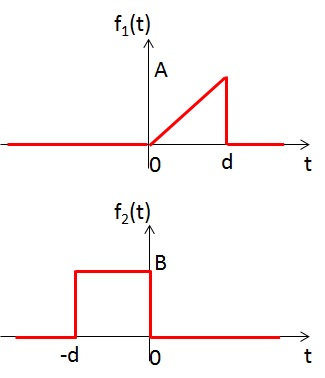
\includegraphics[scale=0.6]{images/Ex_intercorrelation.jpg}
	\end{figure}
	
	Les expressions des deux signaux sont : $f_{1}(t)=\frac{At}{d}(u(t)-u(t-d))$ et $f_{1}(t)=(u(t+d)-u(t))$. Leur produit d'intercorrélation est donné par :
	
	\begin{equation*}
	R_{12}(\tau)=\int_{-\infty}^{+\infty}f_{1}(t)f_{2}(t-\tau)dt
	\end{equation*}
	
	On peut distinguer les quatre intervalles suivants :
	\begin{itemize}
		\item si $\tau < 0$ ou $\tau > 2d$, alors les deux fonctions ne se recouvrent pas et $R_{12}(\tau)=0$.
		\item si $0 \leq \tau < d$, $R_{12}(\tau)=\int_{0}^{\tau}\frac{AB}{d}tdt=\frac{AB}{2d}\tau ^{2}$ 
		\item si $d \leq \tau < 2d$, $R_{12}(\tau)=\int_{\tau-d}^{d}\frac{AB}{d}tdt=\frac{AB}{2d}(d^{2}-(\tau-d)^{2})$
	\end{itemize}
	
	L'allure de la fonction d'intercorrélation est présentée sur la figure ci-dessous. Contrairement à la fonction d'autocorrélation, la fonction d'intercorrélation n'est pas paire et ne passe pas par un maximum à l'origine. Son maximum est atteint lorsqu'on décale le signal $f_{2}$ de +d par rapport à $f_{1}$.


	\begin{figure}[h!]
		\centering
		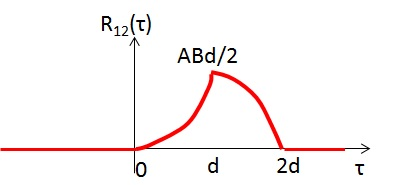
\includegraphics[scale=0.6]{images/Ex_intercorrelation2.jpg}
	\end{figure}
	
	
	\vspace{1\baselineskip}
	
	
	\section{Théorème de Wiener-Khintchine}
	
	Le théorème de Wiener-Khintchine relie la corrélation d'un signal avec sa densité spectrale de puissance. Il fait donc le lien entre une grandeur définie dans le domaine temporel et une autre dans le domaine fréquentiel. Celui-ci peut facilement être démontré en repartant de la formule de la corrélation. Considérons un signal f(t) quelconque, dont l'autocorrélation est donnée par :
	\begin{equation*}
	R_{11}(\tau)=\frac{1}{T}\int_{-\infty}^{+\infty}f(t)f^{*}(t-\tau)dt
	\end{equation*}
	
	On peut exprimer les signaux $f(t)$ et $f(t-\tau)^{*}$ à partir de leur spectre. En utilisant la définition de la transformée de Fourier inverse, on peut montrer que : 
	\begin{equation*}
	f(t)=\int_{-\infty}^{+\infty}F(f)e^{j2\pi ft}df
	\end{equation*}
	\begin{equation*}
	f(t-\tau)^{*}=\int_{-\infty}^{+\infty}F(f)^{*}e^{j2\pi f(t-\tau)^{*}}df=\int_{-\infty}^{+\infty}F(f)^{*}e^{-j2\pi f(t-\tau)}df
	\end{equation*}
	
	En combinant ces différentes équations, on trouve : 
	\begin{equation*}
	R_{11}(\tau)=\frac{1}{T}\int_{-\infty}^{+\infty}[\int_{-\infty}^{+\infty}F(f)e^{j2\pi ft}df][\int_{-\infty}^{+\infty}F(f)^{*}e^{-j2\pi f(t-\tau)}df]dt
	\end{equation*}
	\begin{equation*}
	R_{11}(\tau)=\frac{1}{T}\int_{-\infty}^{+\infty}[\int_{-\infty}^{+\infty}F(f)F(f)^{*}e^{j2\pi f\tau}df]dt
	\end{equation*}
	\begin{equation*}
	R_{11}(\tau)=\int_{-\infty}^{+\infty}F(f)F(f)^{*}e^{j2\pi f\tau}df \cdot \frac{1}{T}\int_{-\infty}^{+\infty}dt
	\end{equation*}
	
	Dans cette dernière expression, on peut remplacer le produit des spectres par la densité spectrale de puissance du signal f(t). La relation \ref{Wiener_Khintchine} correspond au théorème de Wiener-Khintchine.
	
	\begin{equation}\label{Wiener_Khintchine}
		R_{11}(\tau)=\int_{-\infty}^{+\infty}F(f)F(f)^{*}e^{j2\pi f\tau}df=	R_{11}(\tau)=\int_{-\infty}^{+\infty}S_{F}(f)e^{j2\pi f\tau}df
	\end{equation}
	
	L'autocorrélation du signal f(t) n'est rien d'autre que la transformée de Fourier inverse de sa densité spectrale de puissance $S_{F}$. Inversement, on peut affirmer que la densité spectrale de puissance du signal f(t) est la transformée de Fourier de son autocorrélation, comme le montre l'équation \ref{Wiener_Khintchine2}.
	
	\begin{equation}\label{Wiener_Khintchine2}
	S_{F}(f)=	\int_{-\infty}^{+\infty}R_{11}(\tau)e^{-j2\pi f\tau}d\tau
	\end{equation}
	
	
	\vspace{1\baselineskip}
	\textbf{\underline{Cas d'un signal périodique}}
	
	Si le signal est périodique de période $T_{0}$ et de fréquence $F_{0}=\frac{1}{T_{0}}$, le théorème de Wiener-Khintchine est toujours exacte. On peut la réécrire en remplaçant la transformée de Fourier par la série de Fourier. Dans le cas d'une fonction périodique, la notion de densité spectrale de puissance n'a plus de raison d'être, puisque le spectre est constitué de raies portant chacune une partie de la puissance du signal. Le théorème de Wiener-Khintchine relie alors la fonction d'autocorrélation et le spectre de puissance $S_{F}(n)$ du signal. Ces grandeurs sont reliées par les équations \ref{Wiener_Khintchine_periodique} et \ref{Wiener_Khintchine_periodique2}, où n est l'indice d'une raie du spectre.
	\begin{equation}\label{Wiener_Khintchine_periodique}
		R_{11}(\tau) = \sum_{n=-\infty}^{+\infty}S_{F}(n)e^{jn2\pi F_{0}\tau}~,n\in \mathbb{Z}
	\end{equation}
	\begin{equation}\label{Wiener_Khintchine_periodique2}
	S_{F}(n) = \frac{1}{T_{0}}\int_{T_{0}}R_{11}(\tau)e^{jn2\pi F_{0}\tau}d\tau	~,n\in \mathbb{Z}
	\end{equation}
	  
	
	\vspace{1\baselineskip}
	
	Le théorème de Wiener-Khintchine présente un intérêt pratique fort dans la situation suivante. Si on ne dispose pas de l'expression exacte de l'évolution temporelle d'un signal x(t), il est impossible de déterminer celle de sa transformée de Fourier X(f). C'est notamment le cas lorsque l'on traite des signaux aléatoires.	Cependant, si on dispose de l'expression de son autocorrélation, même si on ne peut déterminer la transformée de Fourier du signal, on peut déduire l'expression de la densité spectrale de puissance $S_{X}(f)$ qui est reliée à l'amplitude du spectre du signal $|X(f)|$. L'information de phase du spectre est perdue donc il est impossible de reconstituer le signal temporel. Néanmoins, la densité spectrale de puissance peut être suffisante pour analyser le signal dans le domaine fréquentiel, en montrant comment l'énergie est répartie en fonction de la fréquence. A partir de cette information, un filtre peut être dimensionné pour modifier ou supprimer une partie du contenu fréquentiel du signal, jugée gênante.
	
	\vspace{1\baselineskip}
	
	
	\textbf{\underline{Exemple 1 : spectre de puissance d'un signal cosinusoïdal}} \\
	
	Reprenons l'exemple du signal cosinusoïdale $s(t)=Acos(2\pi f_{0}t+\theta_{0})$ dont on a calculé l'autocorrélation précédemment. Calculez sa transformée de Fourier puis son spectre de puissance. En déduire la fonction d'autocorrélation.
	
	La transformée de Fourier de la fonction s(t) donne :
	\begin{equation*}
	S(f) = \frac{A}{2}e^{j\theta_{0}}\delta(f-f_{0})+\frac{A}{2}e^{-j\theta_{0}}\delta(f+f_{0})
	\end{equation*}
	Son spectre de puissance est donc égale à :
	\begin{equation*}
	S_{F}(f)=|S(f)|^{2}=S(f) \cdot S(f)^{*}=\frac{A^{2}}{4}\delta(f-f_{0})+\frac{A^{2}}{4}\delta(f+f_{0})
	\end{equation*}
	
	On peut remarquer que la puissance moyenne du signal est bien égale à $\frac{A^{2}}{2}$.
	
	L'autocorrélation du signal s(t) peut être déduite du théorème de Wiener-Khitchine, à partir de la transformée de Fourier inverse du spectre de puissance :
	\begin{equation*}
	R_{11}(\tau)=\int_{-\infty}^{+\infty}S_{F}(f)e^{j2\pi f\tau}df=\frac{A^{2}}{2}cos(2\pi f_{0}\tau)
	\end{equation*}
	
	On retrouve l'expression de la fonction d'autocorrélation déterminée dans la partie III.4. \\
	
	
	\textbf{\underline{Exemple 2 : densité spectrale de puissance d'un bruit blanc gaussien}} \\
	
	Reprenons l'exemple du bruit blanc gaussien abordé dans la partie III.3. Sa fonction d'autocorrélation est assimilable à une impulsion de Dirac : $R_{bruit}(\tau) = \sigma^{2}\delta(\tau)$. Comme ce signal est aléatoire, on ne peut pas définir son évolution temporelle par une fonction mathématique. Le calcul de sa transformée de Fourier est donc impossible. Cependant, puisqu'on dispose de sa fonction d'autocorrélation, on peut extraire sa densité spectrale de puissance à l'aide du théorème de Wiener-Khintchine.
	\begin{equation}\label{}
	S_{bruit}(f)=	\int_{-\infty}^{+\infty}R_{bruit}(\tau)e^{-j2\pi f\tau}d\tau
	\end{equation}
	\begin{equation}\label{}
	S_{bruit}(f)=	\int_{-\infty}^{+\infty}\sigma^{2}\delta(\tau)e^{-j2\pi f\tau}d\tau=\sigma^{2}
	\end{equation}
	
	La transformée de Fourier d'une impulsion de Dirac étant une fonction constante en fonction de la fréquence, le spectre d'un bruit blanc est constant quelle que soit la fréquence. On remarque que la puissance moyenne d'un tel signal est infinie et est donc irréalisable dans la pratique. Le bruit blanc que nous avons généré dans la partie III.3 n'est qu'un modèle, discret et à support temporel borné, dont l'énergie est forcément finie.
	
	
	\vspace{1\baselineskip}
	
	
	\section{Relations entre le signal, la densité spectrale de puissance et l'autocorrélation}
	
	Les différentes relations que nous avons vu entre le signal f(t), son spectre F(f), sa densité spectrale de puissance $S_{F}(f$) et son autocorrélation $R_{11}(\tau)$, peuvent être résumées sur la figure \ref{Fig:Relations_f_F_R_S.jpg}. Les flèches à double sens indiquent qu'à partir du spectre du signal, on peut retrouver l'expression du signal et inversement. Même chose pour l'autocorrélation et la densité spectrale de puissance. Cependant, on observe deux flèches à sens unique. La première, entre le signal et son autocorrélation, indique qu'un signal présente une fonction d'autocorrélation unique mais l'inverse n'est pas vraie. La seconde indique qu'on ne peut pas retrouver le spectre d'un signal à partir de sa densité spectrale de puissance. En effet, l'information de phase a été perdue.
	
	\begin{figure}[h!]
		\centering
		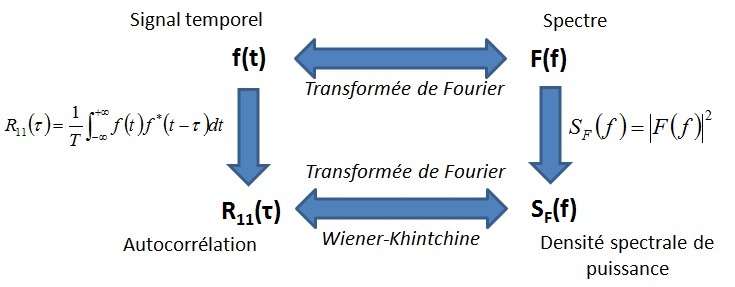
\includegraphics[scale=0.7]{images/Relations_f_F_R_S.jpg}
		\caption{Vue d'ensemble des relations entre le signal, son spectre, sa densité spectrale de puissance et son autocorrélation}	
		\label{Fig:Relations_f_F_R_S.jpg} 
	\end{figure}
	
	


	\section{Transfert d'énergie à travers un système linéaire}
	Avant de terminer ce chapitre, on cherche à savoir comment un système linéaire modifie la densité spectrale de puissance (ou d'énergie) d'un signal apportée sur son entrée. A partir du théorème de Wiener-Khintchine, on pourra aussi déterminer comme le système affecte sa fonction d'autocorrélation.
	
	Prenons le système décrit sur la figure \ref{Fig:Syst_LTI_dsp}. On connait sa réponse impulsionnelle h(t) ou sa fonction de transfert H(f). Un signal x(t) est appliqué sur son entrée, dont on connait la densité spectrale de puissance $S_{X}(f)$. On cherche à déterminer la densité spectrale de puissance $S_{Y}(t)$ du signal de sortie y(t). 
	\begin{figure}[h!]
		\centering
		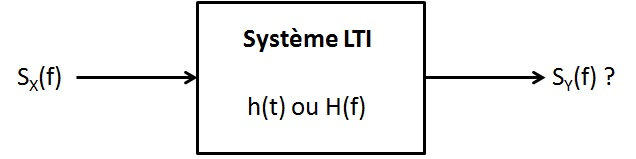
\includegraphics[scale=0.7]{images/Syst_LTI_dsp.jpg}
		\caption{Effet d'un système linéaire sur la densité spectrale de puissance appliquée sur son entrée}	
		\label{Fig:Syst_LTI_dsp} 
	\end{figure}
	
	Le système étant linéaire, les spectres des signaux d'entrée et de sortie sont reliés par l'intermédiaire de la fonction de transfert. A partir de cette relation, on peut exprimer la densité spectrale de puissance de y(t) à partir de celle de y(t). On obtient la relation \ref{dsp_in_out_LTI}. Les densités spectrales de puissance en entrée et en sortie du système sont reliées par de carré du module de sa fonction de transfert.
	\begin{equation*}
	Y(f)=H(f)X(f)
	\end{equation*} 
	\begin{equation}\label{dsp_in_out_LTI}
	S_{Y}(f)=H(f)\cdot H^{*}(f) \cdot |X(f)|^{2}=|H(f)|^{2}S_{X}(f)
	\end{equation}
	
	Cette relation peut être utilisée pour déterminer la fonction d'autocorrélation du signal de sortie $R_{YY}(\tau)$, connaissant celle du signal d'entrée $R_{XX}(\tau)$. Pour cela, on utilise le théorème de Wiener-Khintchine. En notant que la transformée de Fourier inverse d'un produit est un produit de convolution et que $H^{*}(f)=H(-f)$, on obtient la relation \ref{corr_out_dsp}.  
	\begin{equation*}
	R_{YY}(\tau)=\mathcal{F}^{-1}(S_{Y}(f))=\mathcal{F}^{-1}(H(f)H^{*}(f)S_{X}(f))
	\end{equation*}
	\begin{equation*}
	R_{YY}(\tau)=\mathcal{F}^{-1}(H(f))*\mathcal{F}^{-1}(H^{*}(f))*\mathcal{F}^{-1}(S_{X}(f))
	\end{equation*}
	\begin{equation}\label{corr_out_dsp}
	R_{YY}(\tau)=h(\tau)*h(-\tau)*R_{XX}(\tau)
	\end{equation}
	
	\vspace{1\baselineskip}
	
	\section{Exercices}
	
	\subsubsection{Exercice 1}
	
	Calculez la puissance moyenne et l'énergie totale des signaux suivants :\\
	
	a. $\frac{1}{2}+sin(4\pi t)~,~~t \in \mathbb{R}$\\
	
	b. $cos(\pi t)~,~~t \in [0;3]$\\
	
	c. $e^{-t}u(t)~,~~t \in \mathbb{R}$\\
	
	d. Une impulsion rectangulaire, d'amplitude pic-à-pic de 2 V, centrée en -1 V, d'une durée de 0.1 s et de période égale à 1 s.\\
	
	
	\subsubsection{Exercice 2}
	
	\subsubsection{Exercice 2 - Distorsion harmonique}
	
	On dispose du relevé d'un spectre d'amplitude de raies en sortie d'un système (figure ci-dessous à gauche). Le signal est à support temporel non borné.
	
	\begin{figure}[h!]
		\centering
		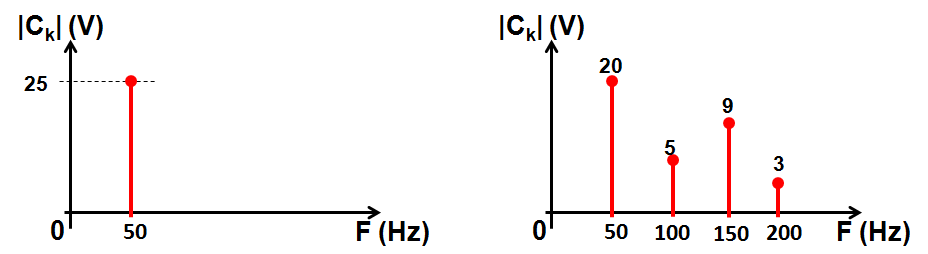
\includegraphics[scale=0.5]{images/Exo_8_2.png} 
	\end{figure}
	
	1. Quelle est la nature du signal ? Précisez ses caractéristiques.\\
	
	2. Quelle est la puissance moyenne du signal ?\\
	
	3. Ce signal traverse un système. On relève le spectre en amplitude en sortie de ce système (figure ci-dessous à droite). Le système est-il linéaire ?\\
	
	4. Calculez la puissance moyenne du signal en sortie du système.\\
	
	5. On définit le taux de distorsion harmonique total (\textit{Total Harmonic Distortion} (THD) en anglais) du signal par rapport au fondamental à l'aide de l'équation suivante :
	\begin{equation*}
	THD_{F}=\frac{\sqrt{\sum_{i=2}^{+\infty}A_{i}^{2}}}{A_{1}}
	\end{equation*}
	
	avec  $A_{i}$ l'amplitude de l'harmonique de rang i. Calculez ce taux sur les signaux d'entrée et de sortie du système.
	
	\vspace{1\baselineskip}
	
	
	\subsubsection{Exercice 3}
	
	1. Soit le signal porte $x(t)=A\cdot \Pi_{\frac{b}{2}(t)}$, $b\in \mathbb{R^{*}}$.
	
	a. Calculez l'énergie totale et la puissance moyenne du signal.
	
	b. Calculez la fonction d'autocorrélation du signal.
	
	c. Calculez la densité spectrale de puissance ou d'énergie
	
	\vspace{0.5\baselineskip}
	
	2. La fonction x(t) est répétée avec une période T pour former le signal f(t). On prendra $b<\frac{T}{2}$.
	
	a. Calculez l'énergie totale et la puissance moyenne du signal.
	
	b. Calculez la fonction d'autocorrélation du signal.
	
	c. Calculez la densité spectrale de puissance ou d'énergie
	
	\vspace{1\baselineskip}
	
	\subsubsection{Exercice 4}
	
	Un signal noté $x(t)=cos(2\pi f_{0}t)$ excite un filtre passe-bas d'ordre 1, dont la fréquence de coupure est $f_{0}$. Le signal en sortie du filtre est noté y(t).
	
	\vspace{0.5\baselineskip}	
	
	1. Donnez l'expression de la transformée de Fourier X(f) du signal x(t). Tracez son module et son argument.
	
	\vspace{0.5\baselineskip}
	
	2. Donnez l'expression de la fonction de transfert H(f) du filtre. Tracez son module et son argument dans le diagramme de Bode. Quel est son gain et son déphasage en $f_{0}$ ?
	
	\vspace{0.5\baselineskip}
	
	3. A partir de X(f) et H(f), déterminez la transformée de Fourier Y(f) du signal y(t).
	
	\vspace{0.5\baselineskip}
	
	4. Déterminez l'expression du signal y(t) à partir de Y(f).
	
	\vspace{0.5\baselineskip}
	
	5. Calculez la puissance moyenne du signal d'entrée. En déduire celle du signal de sortie.
	
	\vspace{1\baselineskip}	
	
	\subsubsection{Exercice 5 - Détection de discontinuité}
	
	On considère un signal x(t) avec plusieurs discontinuités, par exemple : $x(t)=u(t)-2u(t-4)+u(t-6)$. On se propose de trouver une méthode basée sur un calcul d'intercorrélation pour détecter la position de ces discontinuités. On utilise comme signal de détection la fonction $y(t)=sin(2\pi t)(u(t)-u(t-1))$.\\
	
	1. Esquissez l'allure des signaux x(t) et y(t).\\
	
	2. Déterminez l'expression de l'intercorrélation $R_{xy}(\tau)$ entre les signaux x(t) et y(t).Tracez son évolution temporelle. Les discontinuités sont-elles détectées ? Peut-on détecter leur polarité ?\\
	
	3. On choisit un nouveau signal de détection : $y(t)=sin(2\pi \frac{t}{8})(u(t)-u(t-4))$. Reprendre la question précédente. Comment améliorer la précision de la détection ? \\
	
	4. Le dispositif de détection est-il sensible au bruit ?\\
	
	\vspace{1\baselineskip}	
	
	\subsubsection{Exercice 6 - Radar}
	
	La figure ci-dessous illustre le principe de détection d'une cible par le traitement d'un écho radar, et l'estimation de sa distance.
	
	Le radar transmet un signal connu, noté u(t), qui se propage à une vitesse v. Son autocorrélation $R_{u}(\tau)$ est connu. Si un obstacle intercepte ce signal, il en réfléchit une partie. Celle-ci repart en arrière et atteint le radar un temps $t_{1}$ après son émission. Le radar mesure alors l'écho du signal u(t), noté x(t). Celui-ci est la superposition d'une version atténuée du signal u(t) (on supposera l'atténuation constante et on la notera a) et d'un bruit b(t), lié au bruit de mesure et aux interférences électromagnétiques externes.\\
	
	\begin{figure}[h!]
		\centering
		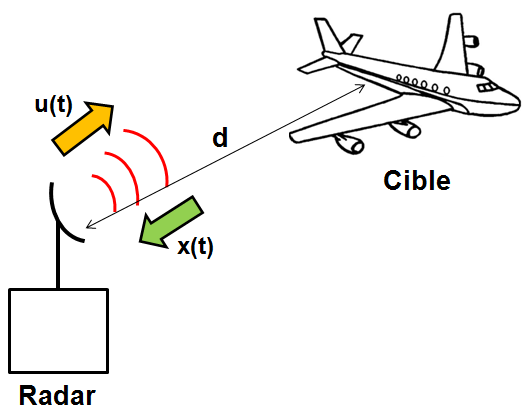
\includegraphics[scale=0.5]{images/TD_8_6.png} 
	\end{figure}
	
	1. Proposez une relation entre les signaux x(t), u(t) et b(t).\\
	
	2. Calculez le produit de convolution : $x(t)*u(-t)$.\\
	
	3. Exprimez l'intercorrélation entre les signaux u(t) et x(t). Exprimez-la en fonction d'autres termes de corrélation.\\
	
	4. Que devient cette expression si le signal de bruit est faiblement corrélé avec le signal u(t) ?\\
	
	5. Proposez une méthode d'estimation de la distance de la cible à partir de la mesure de l'écho du signal radar.\\
	
	6. Quelles propriétés doit vérifier le signal u(t) pour améliorer la précision de la détection ?
	
	
	